\documentclass[11pt]{article}
\usepackage[margin=1.05in]{geometry}
\usepackage{amsmath,amssymb}
\usepackage{booktabs}
\usepackage{enumitem}
\usepackage{graphicx}
\usepackage[font=small,labelfont=bf]{caption}
\usepackage[hidelinks]{hyperref}

\title{Stability Labeling Report:\\ \large Data, Algorithm, Constants, and Results of the FTLE Labeling Campaign}
\author{Aryan Goyal}
\date{July 17, 2026 (updated July 23; reconstructed after the July 21 file loss, see PROGRESS)}

\begin{document}
\maketitle

\begin{abstract}
\noindent
This document inspects the data produced by the stability labeling campaign. It
describes the labeling algorithm in full detail, lists every constant used and where
each constant came from, presents the results for each labeled dataset, explains every
graph and video artifact, and summarizes what proportion of the data falls into each
stability regime and what patterns appear across datasets. As of July 20, about
155{,}000 open-loop stamps are labeled across sixteen datasets from three benchmark
suites (including all ten LIBERO-Long files), and the closed-loop channel is complete
on all four robomimic tasks (lift, can, square, tool\_hang; 3{,}969 stamps). This document is about the labels themselves. Predictor
training and the Stage 1a evaluation, which consume these labels, are documented
separately.
\end{abstract}

\tableofcontents
\newpage

%=====================================================================
\section{What this document covers}

The project needs a per-timestep ground-truth label: is the current moment open-loop
stable (an injected error dies out on its own) or open-loop unstable (an injected
error grows)? A simulator procedure generates these labels. This report documents that
procedure exactly as run, the constants it used, the datasets it was run on, the
resulting label statistics, the sanity-check artifacts (videos and divergence graphs),
and the findings from inspecting all of it. This revision (July 20) adds the
completed LIBERO-Long suite (all ten files) and the finished closed-loop sets for
all four robomimic tasks, tool\_hang included.

%=====================================================================
\section{The two stability measures at a glance}
\label{sec:glance}

In plain terms first. \textbf{Open-loop labels:} take a recorded
demonstration, jump the simulator to some timestep, and run the next 1.2
seconds twice: once replaying the demonstration's recorded actions exactly,
and once replaying the same actions after adding a small error to the first
one, sized like a typical policy mistake. No policy is involved; both runs
are fixed action playback. If the gap between the two trajectories shrinks
or stays flat, the timestep is open-loop stable; if the gap grows, it is
open-loop unstable. This asks ``if one wrong move happens here, does physics
forgive it?'' and it is the primary label, the one the predictor trains on.

\textbf{Closed-loop labels:} the same setup with one change. After the same
injected error, the perturbed run is no longer fixed playback: the trained
diffusion policy looks at its camera observations and picks a fresh action
at every step, reacting as it would at deployment. This is the one place a
trained policy enters the labeling at all, and it was run only after the
Stage 1 policies were fully trained and verified (success 0.9 to 1.0). If
reacting shrinks the gap, the timestep is closed-loop stable; if reacting
makes the gap grow, closed-loop unstable. The channel is a diagnostic, and
its headline finding is that in already-stable regions the policy's own
corrections add error at 90 to 99 percent of stamps, which is the direct
evidence that per-step replanning is harmful there. Ordinary policy
rollouts, the policy running whole episodes, appear only in the Stage 1 and
Stage 2 experiments that measure success rates; they play no part in
labeling.

The rest of this section makes three points precise: what exactly is
perturbed, what differs between the two channels, and whether the channels
are measured at the same places.

\textbf{What is perturbed: an action, never the state.} Neither channel
teleports the simulator state. The perturbation is Gaussian noise on the
position dimensions of the \emph{first commanded action} only (never rotation,
never the gripper), with standard deviation $\sigma_u$ set to the trained
policy's validation action RMSE. The error therefore enters through the
actuation channel, exactly the way a real policy error enters, and becomes a
state deviation only by passing through the plant. What is then \emph{measured}
is in state space: the distance between the perturbed and unperturbed
trajectories in task space over the following 1.2 seconds. So the injection is
in action space, the readout is in state space, and this is identical for both
channels. The channels differ only in what happens after the injection.

\begin{center}
\small
\begin{tabular}{@{}p{0.24\linewidth}p{0.34\linewidth}p{0.34\linewidth}@{}}
\toprule
 & \textbf{Open loop} $\lambda_{ol}$ & \textbf{Closed loop} $\lambda_{cl}$ \\
\midrule
Perturbation & \multicolumn{2}{c}{identical: noise ($\sigma_u$, policy's action
RMSE) on the first action's position dims} \\
\addlinespace
Nominal branch & replays the recorded demo actions & replays the recorded demo
actions \\
\addlinespace
Perturbed branch & replays the same recorded actions; nobody reacts & driven by
the trained policy from its own camera observations, replanning every step \\
\addlinespace
What it isolates & the plant alone: does the task's physics absorb or amplify a
one-time actuation error & the plant plus the policy's feedback loop: does
reacting contain the error or feed it \\
\addlinespace
Readout & \multicolumn{2}{c}{$\lambda$ = OLS slope of branch-averaged log
task-space distance over $K=24$ steps} \\
\addlinespace
Classes & \multicolumn{2}{c}{unstable ($\lambda > +\delta$), stable
($\lambda < -\delta$), deadband ($|\lambda| \leq \delta$)} \\
\addlinespace
Coverage & 200 demos, every 2nd step, $N=8$ branches & 50 demos, every 10th
step, $N=4$ branches \\
\addlinespace
Cost per probe step & one simulator step & one diffusion inference plus one
simulator step (GPU) \\
\addlinespace
Needs a trained policy & no & yes \\
\addlinespace
Role & primary label; the predictor trains on it & diagnostic overlay on the
primary label \\
\bottomrule
\end{tabular}
\end{center}

\textbf{Is closed-loop stability checked where open-loop stability is found?}
Yes, but by construction rather than by conditioning. The closed-loop grid
(demos 0 to 49, every 10th step) is a strict subset of the open-loop grid
(demos 0 to 199, every 2nd step), so every closed-loop stamp has an open-loop
label at the same demonstration and timestep, and the two can be compared
pairwise. The closed-loop probe is run at \emph{every} stamp of its subgrid,
not only where the open-loop label came out stable; gating it on the open-loop
result would have biased the comparison and hidden two of the four scenarios
of Section \ref{sec:scenarios}. The subgrid is a subsample, not the full grid,
purely for cost: every closed-loop probe step is a diffusion-policy inference,
which makes the closed-loop channel roughly two orders of magnitude more
expensive per stamp than the open-loop channel. The reverse containment
therefore does not hold: most open-loop stamps, stable ones included, have no
closed-loop measurement, and the closed-loop claims in this report are claims
about the subsample.

\textbf{All combinations, and the execution each recommends.} Each channel
reports one of three classes, giving nine combinations. The recommended
execution follows from two rules: the open-loop class decides whether
committing is safe (deadband counts as safe to commit, see the deadband
argument in the next section), and the closed-loop class decides whether
reacting helps or hurts. The interesting variation is confined to the
open-loop-unstable row; everywhere else commitment wins.

\begin{center}
\small
\begin{tabular}{@{}lccc@{}}
\toprule
 & CL stable & CL deadband & CL unstable \\
\midrule
OL stable   & commit long $k$ & commit long $k$ & commit long $k$ \\
OL deadband & commit long $k$ & commit long $k$ & commit long $k$ \\
OL unstable & replan per step & short $k$      & intermediate $k$ \\
\bottomrule
\end{tabular}
\end{center}

The reasons per cell, briefly: in the top-right cell replanning is the
destabilizing choice, so commitment is not just cheaper but safer; in the
middle cell the policy is the only error source, so fewer replans mean fewer
errors; in the bottom row, per-step replanning is right only when feedback
genuinely rescues (bottom left), and when both channels are expansive the
best that can be done is an intermediate $k$ that keeps some reaction while
minimizing injected noise.

Empirically the mass concentrates in two cells: transport segments land in
(OL stable or deadband, CL unstable), and contact segments land in
(OL unstable, CL unstable). The rescue cell (OL unstable, CL stable) is rare
in our measurements, and the whole CL-stable column is thin because the
closed-loop channel is positive at 90 to 99 percent of stamps. Section
\ref{sec:scenarios} discusses the four underlying physical scenarios in
detail.

%=====================================================================
\section{The labeling algorithm, in full detail}

\subsection{The quantity being measured}

The label is built from the finite-time Lyapunov exponent (FTLE): the exponential rate
at which a small perturbation grows or shrinks over a short window. The estimator is
the textbook one (Benettin et al.\ 1980): inject a small perturbation, watch the
distance between the perturbed and unperturbed trajectories, and fit the slope of the
log distance against time. A positive slope means the error is amplified (expansive,
unstable). A negative slope means the error is absorbed (contractive, stable).

\subsection{The open-loop probe, step by step}

For each demonstration and each timestep $t_0$ on a stride-2 grid, the labeler runs
the following in the simulator:

\begin{enumerate}[leftmargin=2em]
  \item \textbf{Reset} the simulator to the exact recorded state at $t_0$. All
        datasets used store full simulator states, and replay determinism was
        verified per suite before labeling (Section \ref{sec:suites}).
  \item \textbf{Nominal branch.} Replay the recorded actions
        $a_{t_0}, \dots, a_{t_0+K-1}$ exactly, with $K = 24$ steps (1.2 seconds at
        20 Hz). Record the task-space vector at every step: end-effector position
        concatenated with the object observation vector.
  \item \textbf{Perturbed branches.} Repeat $N = 8$ times: reset to the same state,
        add Gaussian noise with standard deviation $\sigma_u$ to the \emph{position
        dimensions of the first action only} (never rotation, never the gripper),
        then replay the remaining $K-1$ actions unchanged. Nobody reacts; the actions
        are fixed. $\sigma_u$ is set per task to the trained policy's validation
        action RMSE, so the probe injects exactly the size of error the policy
        actually makes at deployment.
  \item \textbf{Divergence.} At every step $\tau = 1..K$, compute
        $d_n(\tau) = \lVert x^{pert}_n(\tau) - x^{nom}(\tau) \rVert$ in task space,
        floor it at $10^{-12}$, and take logs.
  \item \textbf{Slope.} $\lambda(t_0)$ is the ordinary-least-squares slope of the
        branch-averaged $\log d(\tau)$ against $\tau$. A second slope is fitted on
        the full simulator state vector as a secondary channel
        ($\lambda_{\mathrm{full}}$).
  \item \textbf{Contact flags.} At the stamp and over the whole window, record three
        boolean channels: gripper touching the task object, task object touching the
        table, task object touching a fixture (peg, stand, bin, another object).
        Only contacts involving the task object count; distractor-object contacts
        are excluded by per-environment object name patterns. These flags are a
        sanity channel only. The label never uses them.
\end{enumerate}

\subsection{From $\lambda$ to labels and segments}

\begin{itemize}[leftmargin=2em]
  \item $\lambda > +\delta$: \textbf{unstable}. $\lambda < -\delta$: \textbf{stable}.
        $|\lambda| \leq \delta$: \textbf{deadband}, meaning the measured slope is
        within the noise floor and the stamp is unproven either way.
  \item $\delta$ is not a free constant. It is the 95th percentile of $|\lambda|$
        over free-space stamps of the same dataset, i.e.\ the measured noise floor
        of the probe itself. It is computed per dataset.
  \item Deadband stamps inherit the label of their confident neighbors, and a median
        filter over about 3 consecutive stamps smooths the sequence. Contiguous runs
        of one label are the segments. Nothing is ever segmented by hand.
\end{itemize}

\paragraph{Why deadband segments still favor committing $k$ actions.} A deadband
stamp is measured neutrality: the probe injected an error and watched it neither
grow nor shrink, just persist. In such a segment the plant contributes no error of
its own, so the only error source present is the policy, and each replan injects one
fresh policy error that nothing absorbs. Replanning every step therefore accumulates
$T$ injected errors over a $T$-step segment, while committing chunks of $k$ actions
accumulates only $T/k$ of them. Same physics, $k$ times fewer mistakes: commitment
wins in the deadband not despite the uncertainty but because the policy itself is
the dominant noise source there. The lift closed-loop measurement confirms this
directly: at these neutral states, per-step replanning turned the divergence
positive at 99.3\% of stamps while fixed-action replay stayed at zero.

\subsection{Overlapping windows at boundaries between contracting and diverging
regimes}

Stamps sit every 2 steps but each stamp looks 24 steps ahead, so neighboring windows
overlap almost entirely, and a window near a regime boundary can contain both a
contracting stretch and a diverging one. Say contact begins at step 100: the stamp
at step 90 measures a blended slope over 10 stable steps followed by 14 unstable
ones. This is handled deliberately rather than treated as an error. First, the blend
is the honest answer to the question the label asks: committing a chunk at step 90
really is risky, because the contact falls inside the commitment window, so tilting
that stamp toward unstable is correct and gives the controller early warning in the
safe direction. Second, a window that blends the two regimes evenly produces a small
slope, which lands in the deadband rather than forcing a wrong confident call, and
deadband stamps are then resolved by their confident neighbors through inheritance
and the median filter. Third, the probe window $K$ is chosen well below typical
segment length, so mixed windows are confined to the dozen or so stamps nearest each
boundary, and the dense stride brackets the true boundary to within a couple of
steps. The result is that segment edges are slightly early on the way into an
unstable segment and roughly on time on the way out, which is exactly the bias a
safety label should have.

\subsection{The closed-loop variant}

The closed-loop labeler repeats the same probe with one change: after the identical
first-action injection, the perturbed branch is driven by the \emph{trained policy}
acting from its own camera observations with replanning at every step, instead of
replaying the recorded actions. Every probe step is a diffusion-policy inference, so
this channel runs on GPU and on a subsample (stride 10, 50 demos, $N=4$, $K=24$). It
is a diagnostic channel: comparing $\lambda_{cl}$ against $\lambda_{ol}$ per segment
tests the mechanism that feedback injects estimation error where the plant contracts
and corrects error where the plant expands.

\subsection{The four possible scenarios when the two channels are combined}
\label{sec:scenarios}

Each channel classifies a stamp three ways (stable, deadband, unstable), but the
deadband is an abstention, not a third physical regime, so the physically meaningful
question per channel is binary: does the error grow or not? Combining the two
channels then gives exactly four scenarios. All four are logically possible, and
they mean different things and recommend different execution behavior.

\begin{enumerate}[leftmargin=2em]
  \item \textbf{Open loop stable, closed loop stable.} The plant absorbs the
        injected error on its own, and per-step replanning does no harm either.
        Both execution modes are safe, so the tie-break is cost: commit a long
        chunk and save the inference compute. Empirically this scenario is rare
        in our data, because the closed-loop channel is rarely non-positive
        (only 1 to 10 percent of stamps across the four tasks).
  \item \textbf{Open loop stable, closed loop unstable.} The plant absorbs
        committed errors, but the policy's own per-step corrections inject more
        error than they remove. This is the feedback-noise regime, it is the
        dominant scenario in our measurements (68 to 86 percent of open-loop
        stamps sit at or below the deadband while 90 to 99 percent of
        closed-loop stamps are positive), and it is the empirical footing for
        committing long chunks in free space and transport: here replanning is
        not merely unnecessary, it is the destabilizing choice.
  \item \textbf{Open loop unstable, closed loop stable.} The plant amplifies
        committed errors, but reacting corrects them faster than they grow.
        This is the textbook case for short chunks and dense feedback, and it
        is the scenario the switch rule hopes to find at contact boundaries.
        At the stamp level our data shows it is uncommon (even in contact, the
        closed-loop channel stays positive at most stamps), which is itself a
        finding: feedback rescue is not free just because feedback is
        available.
  \item \textbf{Open loop unstable, closed loop unstable.} The plant amplifies
        errors and per-step replanning amplifies them too. Locally, no
        execution mode contains the error; what decides success is whether the
        task funnels the state back (a peg entering its hole is guided by the
        geometry) and how much extra noise each mode injects along the way.
        The Stage 1a rollouts locate contact-heavy segments here and show that
        intermediate chunks (4 to 16 actions) beat per-step replanning in
        them, consistent with divergence data from both channels: when
        nothing is contracting, the winning move is to stop adding feedback
        noise, not to react faster.
\end{enumerate}

Two cautions when reading the table of scenarios. First, the channels measure
state divergence over a 1.2 second window, not task failure; scenario 4 stamps
are frequently crossed successfully by every execution mode, so ``unstable''
means ``sensitive here'', not ``doomed here''. Second, membership is
policy-dependent only through the closed-loop channel: retraining the policy can
move a stamp between scenarios 1 and 2 or between 3 and 4, but never across the
open-loop split, which is a property of the plant alone.

\subsection{Why the primary label replays fixed actions instead of running the policy}

A natural question: would it not be better to let the trained policy act in the
perturbed branch, since the policy is what runs at deployment? No, and for a simple
reason. The label must answer the runtime question ``is it safe to commit a chunk of
actions here without reacting?'' While a chunk is being executed, the robot is by
definition replaying fixed actions, so the safety of committing is a property of the
plant alone, and only the fixed-action probe measures it. The closed-loop probe
answers the other question, ``what happens under per-step replanning?'', and the lift
data shows why it cannot serve as the main label: with the policy reacting,
divergence is positive at 99.3\% of stamps, because the policy's own corrections
inject error even in benign free space. A label built from that would mark nearly
everything unstable and recommend per-step replanning everywhere, which is exactly
the failure mode the theory warns against. There is also a practical reason: the
fixed-action label is a property of the robot, controller, and environment, so it
stays valid when the policy is retrained or replaced, while a policy-in-the-loop
label would have to be regenerated with every new checkpoint. The closed-loop
channel is therefore kept as a separate diagnostic: the open-loop label licenses
committing, and the closed-loop label tells us whether reacting helps where
committing is unsafe.

\subsection{Which labels need a trained policy, and which do not}
\label{sec:policy-dependency}

A reasonable worry: labeling ran while policy trainings were still in
progress, so how could the labels exist before the policies did? The answer
is that the two label channels have different inputs, and only one of them
involves a policy at all.

\begin{itemize}[leftmargin=2em]
  \item \textbf{The open-loop channel needs no policy.} Its probe perturbs a
        state and then replays the \emph{recorded demonstration actions} on
        both branches. Everything it touches (the demonstrations, the
        simulator, the perturbation) exists the moment a dataset is
        downloaded. This is the primary label, it is what the predictor is
        trained on, and it was generated for every dataset in this report
        with no policy in the loop. It is also why the label stays valid
        when a policy is retrained or replaced.
  \item \textbf{The closed-loop channel does need a trained policy}, because
        its perturbed branch is driven by policy inference. It was therefore
        generated last, and only for the four robomimic tasks, using the
        finished Stage 1 policies (lift epoch 100 and can epoch 1050 at
        success 1.0, square epoch 950 at 0.9, tool\_hang epoch 1200 at 0.9).
        Nothing downstream trains on it; it is a diagnostic overlay on the
        open-loop label.
\end{itemize}

Concretely for Stage 2: the four MimicGen long-horizon tasks have no labels
and, on the current plan, need none, because the predictor head is applied
zero-shot. If zero-shot transfer underperforms, the fallback is to label
MimicGen demonstrations with the open-loop probe, and that fallback again
waits on nothing, because it replays demonstration actions rather than
querying the Stage 2 policies. At no point is any labeling blocked on a
training run.

\subsection{Why do we need a predictor or oracle at all?}

The labels in this report are indexed by demonstration and timestep. But at
execution time the robot creates a brand new trajectory of its own, visiting states
that sit on no demonstration's timeline, so there is no table to look the answer up
in. The stability of the current moment has to be judged live. Inside the simulator
we can do that exactly: freeze the state, run the perturb-and-replay probe, and read
off $\lambda$; this is the oracle used in the Stage 1a experiments, and it exists to
test whether the switching rule helps when given perfect information. A real robot,
however, cannot freeze time and rewind itself to measure its own divergence. The
only stability-relevant signal available at deployment is what the robot can see:
the last second or two of camera frames. The predictor exists purely to read the
regime out of those frames, approximating the oracle that the labels in this report
define. If the oracle rule does not help, no predictor can; if it does, the
predictor is what carries the rule out of the simulator.

\subsection{Per-suite protocol differences and determinism findings}
\label{sec:suites}

Replay determinism is the hard prerequisite: the same reset plus the same actions must
give the same trajectory, or the divergence measurement is meaningless. Findings per
suite:

\begin{itemize}[leftmargin=2em]
  \item \textbf{robomimic (lift, can, square, tool\_hang).} Runs in the main stack
        (robosuite 1.5.1, mujoco 3.2.6). Replay is bit-exact. Labeling uses the
        robomimic EnvRobosuite path with the per-demo model XML restored first.
  \item \textbf{MimicGen (stack\_d0, square\_d0).} MimicGen environments require the
        robosuite 1.4 API, so labeling runs in a dedicated environment (robosuite
        1.4.1, mujoco 2.3.2, robomimic v0.3 with a small legacy-import patch).
        Replay does NOT match the \emph{stored} states exactly (a decaying joint
        velocity transient of about 0.1 at the first step, an artifact of the warm
        controller state during data generation), but replay
        \emph{self-consistency} is bit-exact, which is what the probe needs: nominal
        and perturbed branches share any transient, and it cancels in the
        divergence.
  \item \textbf{LIBERO (libero\_10, the LIBERO-Long suite).} Replay is deterministic
        only through LIBERO's native environment wrapper (its
        \texttt{set\_init\_state} forces observable and post-process updates that the
        generic path skips), and only from the second rollout after a context change
        onward. The labeler therefore runs one warm-up rollout per stamp and
        discards it; after that, repeats are bit-exact (max difference
        $1.5\times10^{-15}$ over 16 steps). A dedicated labeler entrypoint
        implements this protocol. The task-space metric for LIBERO is the
        end-effector site position plus all free-joint object poses.
  \item \textbf{FurnitureSim.} Blocked: its simulator requires Isaac Gym, which is
        not installable without a manual NVIDIA-login download. No labels yet.
\end{itemize}

%=====================================================================
\section{Constants used, and where each one came from}

\begin{center}
\begin{tabular}{@{}lll@{}}
\toprule
Constant & Value & Provenance \\
\midrule
Probe window $K$ & 24 steps (1.2 s) & probe study; bracketed by fit/decision \\
 & & lower bounds and locality/saturation \\
 & & upper bounds (plan doc, Choosing K) \\
Branches $N$ & 8 & probe study; slope variance acceptable \\
Stride & every 2 steps & label density vs cost \\
Perturbed dims & position only (3 of 7) & probe study: rotation noise injects \\
 & & lever-arm noise that swamps free space \\
Gripper perturbation & never & binary channel, not an error model \\
$\sigma_u$ lift & 0.1651 & measured: policy validation pos-RMSE \\
$\sigma_u$ can & 0.2251 & measured \\
$\sigma_u$ square & 0.2201 & measured \\
$\sigma_u$ tool\_hang & 0.1638 & measured \\
$\sigma_u$ MimicGen square\_d0 & 0.2201 & borrowed from square (same task family) \\
$\sigma_u$ MimicGen stack\_d0 & 0.203 & mean of the three measured values; interim \\
$\sigma_u$ LIBERO (all) & 0.203 & robomimic mean; interim until a LIBERO \\
 & & policy is trained \\
Deadband $\delta$ & per dataset, 0.017--0.052 & p95 of $|\lambda|$ over free-space stamps \\
Median filter & $\sim$3 stamps & boundary smoothing \\
Divergence floor & $10^{-12}$ & numerical guard before log \\
CL subsample & stride 10, 50 demos, $N{=}4$ & cost: every step is a diffusion inference \\
\bottomrule
\end{tabular}
\end{center}

The earlier labeling pass used a placeholder $\sigma_u = 0.05$ for all tasks. The
measured values are 3 to 4.5 times larger. All robomimic labels reported here were
regenerated with the measured values; the change matters (Section
\ref{sec:patterns}).

%=====================================================================
\section{The datasets labeled}

\begin{center}
\footnotesize
\begin{tabular}{@{}llrrll@{}}
\toprule
Suite & Dataset & Demos & Stamps & $\sigma_u$ (source) & Status \\
\midrule
robomimic & lift-ph & 200 & 2{,}485 & 0.165 (measured) & done \\
robomimic & can-ph & 200 & 9{,}254 & 0.225 (measured) & done \\
robomimic & square-ph & 200 & 12{,}723 & 0.220 (measured) & done \\
robomimic & tool\_hang-ph & 200 & 45{,}633 & 0.164 (measured) & done \\
MimicGen & stack\_d0 & 200 of 1000 & 8{,}445 & 0.203 (interim) & done \\
MimicGen & square\_d0 & 200 of 1000 & 12{,}874 & 0.220 (borrowed) & done \\
LIBERO-Long & KITCHEN\_SCENE3 (stove+moka) & 50 & 6{,}060 & 0.203 (interim) & done \\
LIBERO-Long & KITCHEN\_SCENE4 (bowl in cabinet) & 50 & 5{,}632 & 0.203 (interim) & done \\
LIBERO-Long & KITCHEN\_SCENE6 (two mugs) & 50 & 7{,}031 & 0.203 (interim) & done \\
LIBERO-Long & KITCHEN\_SCENE8 (two moka pots) & 50 & 9{,}812 & 0.203 (interim) & done \\
LIBERO-Long & LIVING\_ROOM\_SCENE1 (soup+cheese) & 50 & 6{,}147 & 0.203 (interim) & done \\
LIBERO-Long & LIVING\_ROOM\_SCENE2 (soup+sauce) & 50 & 6{,}761 & 0.203 (interim) & done \\
LIBERO-Long & LIVING\_ROOM\_SCENE2 (cheese+butter) & 50 & 5{,}920 & 0.203 (interim) & done \\
LIBERO-Long & LIVING\_ROOM\_SCENE5 (mug on plate) & 50 & 5{,}868 & 0.203 (interim) & done \\
LIBERO-Long & LIVING\_ROOM\_SCENE6 (mug+pudding) & 50 & 5{,}789 & 0.203 (interim) & done \\
LIBERO-Long & STUDY\_SCENE1 (book in caddy) & 50 & 4{,}146 & 0.203 (interim) & done \\
robomimic CL & lift (closed loop) & 50 & 151 & 0.165 & done \\
robomimic CL & can (closed loop) & 50 & 477 & 0.225 & done \\
robomimic CL & square (closed loop) & 50 & 644 & 0.220 & done \\
robomimic CL & tool\_hang (closed loop) & 50 & 2{,}697 & 0.164 & done \\
\bottomrule
\end{tabular}
\end{center}

Total labeled: about 155{,}000 open-loop stamps across sixteen datasets (four
robomimic, two MimicGen, all ten LIBERO-Long files), plus four finished closed-loop
sets (lift, can, square, tool\_hang; 3{,}969 stamps). Label generation cost:
roughly 15 to 60 minutes per dataset on CPU workers for open loop; about 9 to 13
hours per task for the closed-loop channel because every probe step is a policy
inference (tool\_hang, with the longest episodes, took 53.6 hours).

%=====================================================================
\section{Results per dataset}

Each dataset below reports: the $\lambda$ distribution (mean, 5th, 50th, 95th
percentile), the regime proportions after thresholding (unstable / stable /
deadband), the contact-alignment AUROC (how well $\lambda$ ranks
contact-in-window, the sanity check), the per-contact-category mean $\lambda$, and
the deadband $\delta$. All numbers use the true measured or interim $\sigma_u$ as
listed above.

\subsection{robomimic}

\paragraph{lift-ph.}
2{,}485 stamps. $\lambda$: mean $+0.036$, p5 $-0.012$, median $+0.015$, p95
$+0.184$. Regimes: 30.6\% unstable, 0.0\% stable, 69.4\% deadband
($\delta = 0.025$). AUROC 0.86, the best of the robomimic set. Mean $\lambda$ under
gripper contact is $+0.073$, about five times the overall median. Reading: lift is
short and simple; the grasp moment is sharply expansive and everything else is
neutral. The absence of confidently stable stamps is discussed in Section
\ref{sec:patterns}.

\paragraph{can-ph.}
9{,}254 stamps. $\lambda$: mean $+0.019$, p5 $-0.032$, median $+0.009$, p95
$+0.115$, the mildest distribution of the four. Regimes: 12.5\% unstable, 1.1\%
stable, 86.4\% deadband. AUROC undefined by construction: the can rests in a bin
from the first frame (object-fixture contact in every window) and is gripped
afterward, so there are no contact-free stamps to rank against. $\delta$ falls back
to 0.05, close to square's measured 0.041. Reading: can is confirmed as the
mostly-stable control task; it has the lowest unstable fraction of any dataset
labeled.

\paragraph{square-ph.}
12{,}723 stamps. $\lambda$: mean $+0.031$, p5 $-0.026$, median $+0.017$, p95
$+0.128$. Regimes: 31.1\% unstable, 1.0\% stable, 67.9\% deadband
($\delta = 0.041$). AUROC 0.72. Mean $\lambda$: fixture contact $+0.050$ versus
gripper contact $+0.041$; the peg-insertion phase is the most expansive part of the
task, as expected.

\paragraph{tool\_hang-ph.}
45{,}633 stamps, the largest labeled set (longest episodes, 240px scenes). $\lambda$:
mean $+0.032$, p5 $-0.025$, median $+0.026$, p95 $+0.114$. Regimes: 30.1\% unstable,
0.3\% stable, 69.5\% deadband ($\delta = 0.046$). AUROC 0.86. Fixture contact mean
$+0.041$ versus gripper $+0.038$. Reading: tool\_hang is contact-heavy (93\% of
windows contain a task-object contact) and its label structure is the cleanest of
the hard tasks, which supports its role as a primary hypothesis-test task.

\subsection{MimicGen}

\paragraph{stack\_d0.}
8{,}445 stamps from the first 200 of 1000 generated demos. $\lambda$: mean $+0.028$,
median $+0.019$, p95 $+0.115$. Regimes: 29.1\% unstable, 0.2\% stable, 70.7\%
deadband ($\delta = 0.030$). AUROC 0.73. Fixture contact mean $+0.062$, the highest
fixture value measured: cube-on-cube placement is a sharply expansive event.

\paragraph{square\_d0.}
12{,}874 stamps. $\lambda$: mean $+0.032$, median $+0.020$, p95 $+0.122$. Regimes:
25.5\% unstable, 0.3\% stable, 74.2\% deadband ($\delta = 0.052$). AUROC 0.75.
Fixture mean $+0.055$ versus gripper $+0.043$. Reading: MimicGen square reproduces
the human-demo square's structure closely (compare 31\%/0.72 above), which is
evidence that generated demos carry the same stability anatomy as human ones. This
matters because MimicGen is the cheap-scale path for predictor training data.

\subsection{LIBERO-Long (all ten files)}

All ten LIBERO-Long task files are now labeled: 63{,}166 stamps, the largest suite
in the campaign. One protocol note first. The deadband rule needs contact-free
stamps to estimate the noise floor, and in six of the ten scenes (the five
living-room files and the study file) the generic contact patterns fire in every
single window, so those scenes have no free-space stamps at all. For them $\delta$
falls back to the suite-level value $0.019$, computed by pooling the 7{,}527
free-space stamps that exist across the four kitchen scenes. The four kitchen
scenes use their own per-scene $\delta$ (0.017 to 0.020), consistent with the
values already reported. The same all-contact problem makes the contact-alignment
AUROC undefined for those six scenes: there is no contact-free class to rank
against, exactly as with can.

\begin{center}
\footnotesize
\begin{tabular}{@{}lrccccc@{}}
\toprule
Task file & Stamps & mean $\lambda$ & p95 & Unstable & Stable & AUROC \\
\midrule
KITCHEN\_SCENE3 (stove+moka) & 6{,}060 & $+0.012$ & $+0.082$ & 22.7\% & 12.3\% & 0.42 \\
KITCHEN\_SCENE4 (bowl in cabinet) & 5{,}632 & $+0.028$ & $+0.110$ & 36.8\% & 3.6\% & 0.60 \\
KITCHEN\_SCENE6 (two mugs) & 7{,}031 & $+0.031$ & $+0.111$ & 36.3\% & 1.2\% & 0.63 \\
KITCHEN\_SCENE8 (two moka pots) & 9{,}812 & $+0.024$ & $+0.094$ & 28.1\% & 2.0\% & 0.54 \\
LIVING\_ROOM\_SCENE1 (soup+cheese) & 6{,}147 & $+0.026$ & $+0.116$ & 28.4\% & 3.5\% & -- \\
LIVING\_ROOM\_SCENE2 (soup+sauce) & 6{,}761 & $+0.032$ & $+0.127$ & 34.7\% & 2.0\% & -- \\
LIVING\_ROOM\_SCENE2 (cheese+butter) & 5{,}920 & $+0.031$ & $+0.132$ & 30.6\% & 1.3\% & -- \\
LIVING\_ROOM\_SCENE5 (mug on plate) & 5{,}868 & $+0.037$ & $+0.130$ & 42.1\% & 2.3\% & -- \\
LIVING\_ROOM\_SCENE6 (mug+pudding) & 5{,}789 & $+0.034$ & $+0.134$ & 36.5\% & 2.4\% & -- \\
STUDY\_SCENE1 (book in caddy) & 4{,}146 & $+0.024$ & $+0.089$ & 21.4\% & 1.4\% & -- \\
\midrule
Suite total & 63{,}166 & & & 31.9\% & 3.1\% & \\
\bottomrule
\end{tabular}
\end{center}

The remainder in every row is deadband; the suite splits 31.9\% unstable, 3.1\%
stable, 65.0\% deadband, which is squarely in the robomimic range. Note the small
per-scene differences against the three files reported while labeling was still
running (for example SCENE3 was quoted as 21.4\%/11.8\%): those earlier numbers
used the labeler's in-flight analysis pass; the table above recomputes every file
with one uniform rule and supersedes them.

\paragraph{Reading, and an honest flag.} The $\lambda$ distributions look like the
robomimic ones (slightly positive median, strong positive tail). SCENE3 remains the
only dataset in the whole campaign with a substantial confidently-stable fraction
(12.3\%), and the two-object living-room tasks are the most unstable-heavy sets
labeled anywhere (up to 42.1\%), which fits their anatomy: two full
pick-place cycles per episode. But the sanity channel is weak here: where the
contact-alignment AUROC is computable at all it spans 0.42 to 0.63, clearly below
robomimic and MimicGen (0.72 to 0.86), and in six scenes it is not computable
because generic contact patterns saturate. Two known causes: the contact-flag
implementation for LIBERO uses generic name patterns rather than per-scene
task-object patterns, so the sanity channel itself is noisy in multi-object scenes;
and $\sigma_u$ is an interim borrowed value because no LIBERO policy exists yet.
The $\lambda$ values themselves are measured with the same verified-deterministic
probe; it is the alignment check that is degraded, not necessarily the labels.
Treat LIBERO labels as provisional until per-scene contact patterns and a measured
$\sigma_u$ exist. This is listed in Caveats (Section \ref{sec:caveats}).

\subsection{Closed-loop channel (all four tasks complete)}

All four closed-loop sets are complete, with 50 demos at stride 10:

\begin{center}
\small
\begin{tabular}{@{}lrcccc@{}}
\toprule
Task & Stamps & mean $\lambda_{cl}$ & p5 & p95 & $\lambda_{cl} > 0$ \\
\midrule
lift        & 151     & $+0.092$ & $+0.015$ & $+0.202$ & \textbf{99.3\%} \\
can         & 477     & $+0.080$ & $-0.012$ & $+0.221$ & \textbf{90.4\%} \\
square      & 644     & $+0.090$ & $-0.009$ & $+0.231$ & \textbf{93.0\%} \\
tool\_hang  & 2{,}697 & $+0.096$ & $+0.013$ & $+0.228$ & \textbf{97.6\%} \\
\bottomrule
\end{tabular}
\end{center}

Compare the open-loop labels on the same tasks: means $+0.019$ to $+0.036$, with 68
to 86 percent of stamps in the deadband. On the same states, with the same injected
error: fixed-action replay mostly absorbs or carries the error (open loop), while
per-step policy replanning makes the divergence grow at 90 to 99 percent of stamps
(closed loop). The mechanism the whole hypothesis rests on is now confirmed on
three tasks, not one: in segments where the plant does not amplify errors, the
policy's own feedback does. Two details are worth noting. First, the effect is
strongest on lift (99.3\%), the most benign plant, which is exactly the prediction:
the more neutral the plant, the more the feedback injection dominates the measured
divergence. Second, can, the mostly-stable control task with the mildest open-loop
distribution (12.5\% unstable), still shows 90.4\% positive closed-loop stamps; even
the easiest task cannot absorb per-step replanning noise. Third, tool\_hang, the most
contact-heavy task (93 percent of stamps in contact), lands at 97.6 percent
positive with the largest mean ($+0.096$): the harder the contact regime, the
closer the closed-loop channel gets to uniformly expansive. This state-level
result has a rollout-level counterpart: in the Stage 1a evaluation (separate
report, now pooled over three seeds), replanning every step during contact costs
0.14 to 0.21 in success rate on tool\_hang against committing 4 or 16 actions,
at three to five sigma.

%=====================================================================
\section{Cross-dataset patterns and insights}
\label{sec:patterns}

\begin{figure}[t]
\centering
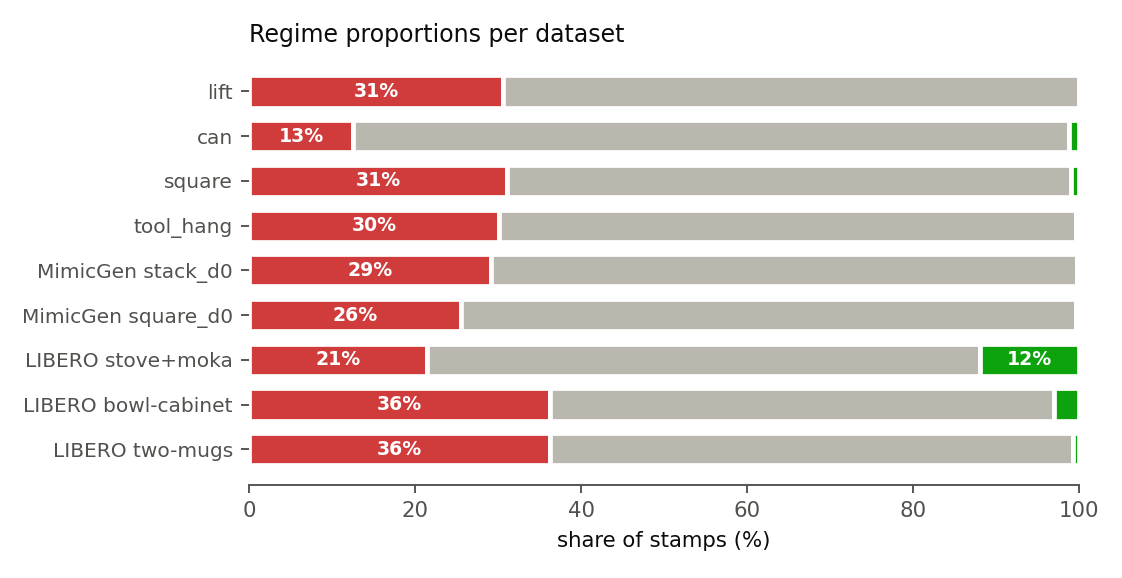
\includegraphics[width=0.95\linewidth]{figs/fig_regimes.png}
\caption{Regime proportions per dataset after thresholding. Red is unstable
($\lambda > +\delta$), gray is deadband ($|\lambda| \leq \delta$), green is stable
($\lambda < -\delta$); segments are in that fixed order, with the percentage printed
on any segment large enough to hold it. Two outliers carry the message: can (the
designated mostly-stable control) has by far the smallest red share, and the LIBERO
stove task is the only dataset with a visible green share (the knob-turning phase is
mechanically guided).}
\label{fig:regimes}
\end{figure}

\begin{figure}[t]
\centering
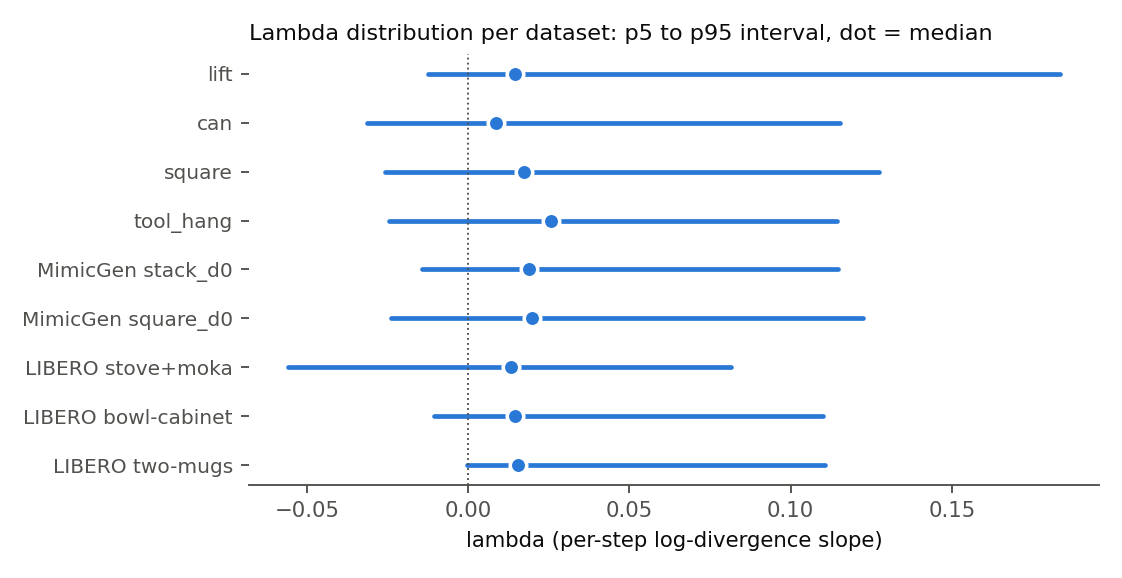
\includegraphics[width=0.95\linewidth]{figs/fig_lambda_dist.png}
\caption{The $\lambda$ distribution per dataset: the bar spans the 5th to 95th
percentile, the dot is the median. Every dataset shows the same one-sided shape: a
median just above zero, a short left tail (weak contraction at most), and a long
right tail (strong expansion). The label information lives in that right tail.}
\label{fig:lamdist}
\end{figure}

\paragraph{1. Regime proportions are remarkably consistent
(Figure~\ref{fig:regimes}).}
Across every suite, roughly one quarter to one third of stamps are confidently
unstable, nearly none are confidently stable, and two thirds to three quarters sit
in the deadband:

\begin{center}
\begin{tabular}{@{}lrrr@{}}
\toprule
Dataset & unstable & stable & deadband \\
\midrule
lift & 30.6\% & 0.0\% & 69.4\% \\
can & 12.5\% & 1.1\% & 86.4\% \\
square & 31.1\% & 1.0\% & 67.9\% \\
tool\_hang & 30.1\% & 0.3\% & 69.5\% \\
MimicGen stack\_d0 & 29.1\% & 0.2\% & 70.7\% \\
MimicGen square\_d0 & 25.5\% & 0.3\% & 74.2\% \\
LIBERO SCENE3 & 21.4\% & 11.8\% & 66.7\% \\
LIBERO SCENE4 & 36.2\% & 3.0\% & 60.8\% \\
LIBERO SCENE6 & 36.3\% & 0.7\% & 63.1\% \\
\bottomrule
\end{tabular}
\end{center}

The exception on both ends is instructive: can (the designated mostly-stable
control) has by far the fewest unstable stamps, and LIBERO SCENE3 (stove knob
turning, a guided articulated mechanism) has the only large stable fraction.

\paragraph{2. The label distribution is one-sided: red islands in a gray sea
(Figure~\ref{fig:lamdist}).}
Confidently stable stamps are nearly absent everywhere. The reason is physical, not
a bug: with a stiff operational-space controller, a position error in free space
neither grows nor actively shrinks in task space within 1.2 seconds; it persists.
Persistence is $\lambda \approx 0$, which is the deadband. Active contraction
(errors visibly funneling in) is rare in these plants at this probe scale. The
informative signal is therefore the sign boundary between "unstable" and
"everything else", and the final segments come from unstable islands plus
neighbor-inheritance over the gray.

\begin{figure}[t]
\centering
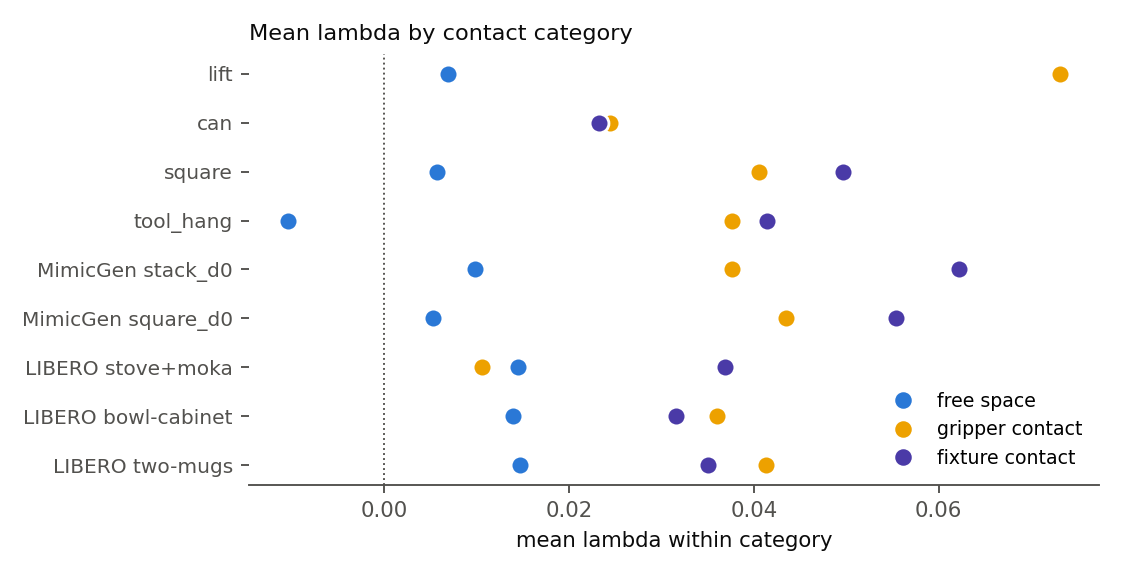
\includegraphics[width=0.95\linewidth]{figs/fig_contact_lambda.png}
\caption{Mean $\lambda$ by contact category. In every dataset where all three
categories exist, the ordering is the same: fixture contact (violet, insertion and
placement events) is the most expansive, gripper contact (yellow) next, free space
(blue) lowest and nearest zero. The hardest physical moments are measurably the most
error-amplifying.}
\label{fig:contact}
\end{figure}

\paragraph{3. Contact category orders $\lambda$ the same way in every dataset
(Figure~\ref{fig:contact}).}
Fixture contact (insertion, placement, object-on-object) has the highest mean
$\lambda$, gripper contact is next, and free space is lowest, in every dataset where
all three exist. Examples: stack\_d0 fixture $+0.062$ vs gripper $+0.038$; square
$+0.050$ vs $+0.041$; square\_d0 $+0.055$ vs $+0.043$. The physically hardest
moments (parts touching parts) are measurably the most error-amplifying, which is
exactly what the adaptive-chunking hypothesis needs to be true.

\paragraph{4. The size of the injected error matters, so measuring $\sigma_u$
mattered.} Regenerating robomimic labels with the measured $\sigma_u$ (3 to 4.5
times the placeholder) moved the unstable fraction from roughly 18--22\% to
25--31\% and cut the deadbands roughly in half on lift and square. Probing with an
unrealistically small error understates how much of the task is dangerous for the
policy that will actually run.

\paragraph{5. Generated demos have the same stability anatomy as human demos.}
MimicGen square\_d0 versus human square-ph: unstable fraction 25.5\% vs 31.1\%,
AUROC 0.75 vs 0.72, the same fixture-above-gripper ordering, nearly the same p95.
This supports using MimicGen for cheap predictor-training scale.

\begin{figure}[t]
\centering
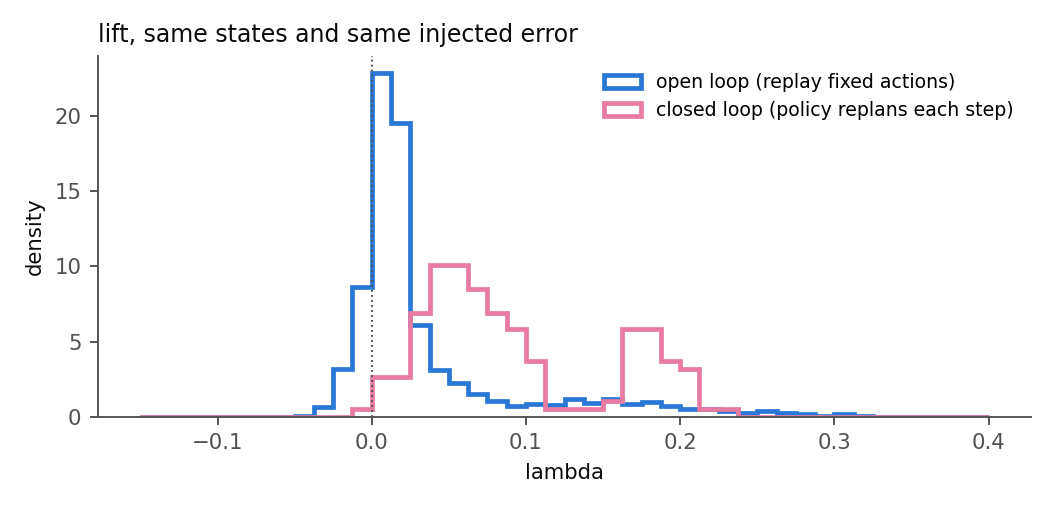
\includegraphics[width=0.85\linewidth]{figs/fig_ol_vs_cl_lift.png}
\caption{The closed-loop mechanism check on lift. Both histograms measure the same
states with the same injected error size. Open loop (blue): replaying the fixed
recorded actions leaves $\lambda$ concentrated at zero; the plant mostly carries the
error without amplifying it. Closed loop (magenta): letting the policy replan every
step shifts the whole distribution positive (99.3\% of stamps), with a second mode
near $+0.2$. The policy's own corrections are the source of divergence in this
mostly-benign task, exactly the feedback-injects-error mechanism the theory
predicts.}
\label{fig:olcl}
\end{figure}

\paragraph{6. The closed-loop mechanism check now passes on all four tasks
(Figure~\ref{fig:olcl}).} On lift, $\lambda_{cl} > 0$ at 99.3\% of stamps; on can,
90.4\%; on square, 93.0\%; on tool\_hang, 97.6\%; while the open-loop labels on
the same tasks are mostly neutral. Feedback injects error where the plant would
have carried it, and it does so on every task labeled, from the mildest (can) to
the most contact-heavy (tool\_hang). This is the Section-1 mechanism of the
hypothesis observed in measured data, four times independently.

\paragraph{7. Label noise at the extremes is real and quantified.} Re-measuring
hand-picked extreme stamps with fresh random branches reproduces the sign but not
always the magnitude (one tool\_hang stamp: label $+0.31$, recomputation $+0.07$).
Slopes deep in the tail are order-of-magnitude estimates, not precise rates. The
binary label is robust; the auxiliary $\lambda$ regression target carries tail
noise, which is why it is weighted as an auxiliary loss, not the decision loss.

\paragraph{8. Free space measures neutral, not contractive, and this agrees with
the theory literature once the perturbed quantity is stated carefully.} Across all
sixteen datasets, free-space $\lambda$ concentrates at zero: injected errors
persist rather than decay. This is a consequence of what the probe perturbs. We
perturb the \emph{action} (the commanded target), and the low-level position
controller then faithfully tracks the shifted command; there is no restoring force
pulling the perturbed trajectory back to the nominal one. Genuinely negative
$\lambda$ requires a physical funnel (a chamfer guiding a peg, a closing grasp
centering an object), and such funneling moments are rare and brief in these
demonstrations, which is why confidently stable fractions are 0 to 3 percent
almost everywhere (LIBERO KITCHEN\_SCENE3, with its constrained stove-knob motion,
is the one exception at 12 percent).

We checked whether this contradicts the imitation-learning stability literature,
and it does not. In Block, Simchowitz, and Tedrake, ``Provable Guarantees for
Generative Behavior Cloning'' (arXiv:2307.14619), incremental stability is not
claimed as a natural property of robot motion: it is \emph{provided} by
synthesized low-level primitive controllers (affine gains stabilizing the
Jacobian linearization around each demonstration), the paper locates the
stabilization ``either learned or implicit in position-command control,'' and it
stresses that access to these synthesized gains ``is a stronger requirement than
classical behavior cloning.'' Moreover their stability notion lets differences in
\emph{initial state} decay over time, while action perturbations
$\delta u$ enter only through a bounded tube $\gamma(\max_t \|\delta u_t\|)$:
bounded, not decaying. Likewise, ``The Pitfalls of Imitation Learning when
Actions are Continuous'' (Simchowitz et al., arXiv:2503.09722) \emph{assumes}
exponential incremental input-to-state stability as a benign theoretical setting,
in which state differences decay as $C\rho^t$ but input differences accumulate
additively; the paper makes no empirical claim that real free-space robot motion
is contractive. So the literature says state errors can be servoed away by a
low-level controller, and says nothing about action errors dying out on their
own. Our probe measures exactly the action-error case, and finds it neutral. The
two pictures are consistent, and together they support the design premise shared
by both this project and that line of work: committing chunks of actions is safe
where the open-loop dynamics do not amplify errors, and the amplification, when
it comes, comes from contact.

%=====================================================================
\section{Per-demonstration label timelines: are the labels long-horizon?}
\label{sec:timelines}

A predictor-driven switch is only useful if the labels form segments a
controller could act on. If the classes alternated stamp to stamp (salt and
pepper), no switching policy could follow them and the whole premise would be
in doubt. This section makes that checkable by eye: for every labeled
demonstration of the four robomimic tasks, one row per demonstration, timestep
on the horizontal axis, and the three-class label at every stamp drawn as a
colored block spanning its subsample stride (open-loop stride 2, closed-loop
stride 10). Blue is stable ($\lambda < -\delta$), light gray is the deadband
($|\lambda| \leq \delta$), red is unstable ($\lambda > \delta$), with
$\delta = 0.0355$ for both channels, and white is past the end of the
demonstration.

\begin{center}
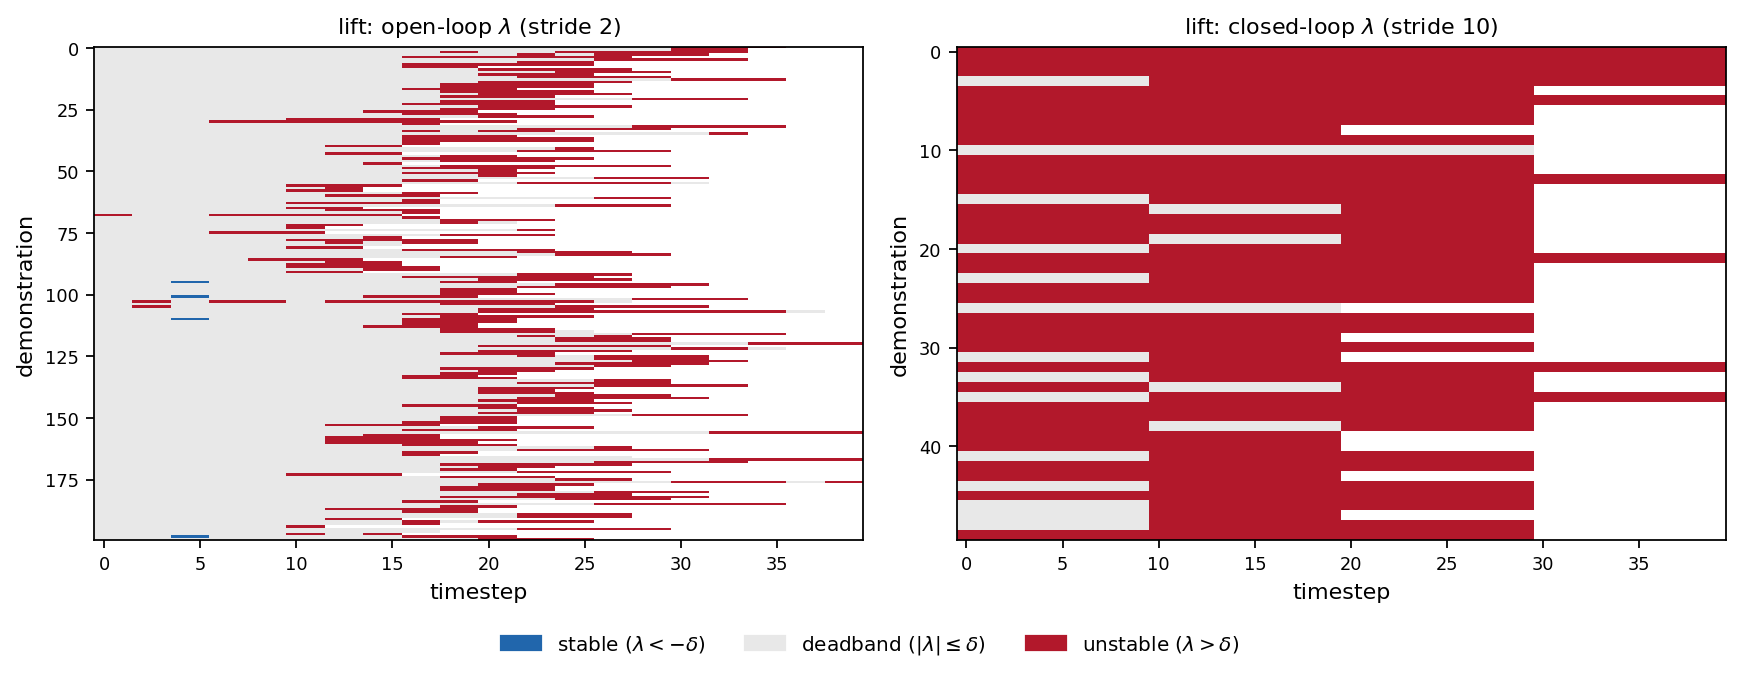
\includegraphics[width=0.98\linewidth]{figs/timeline_lift.png}\\[2pt]
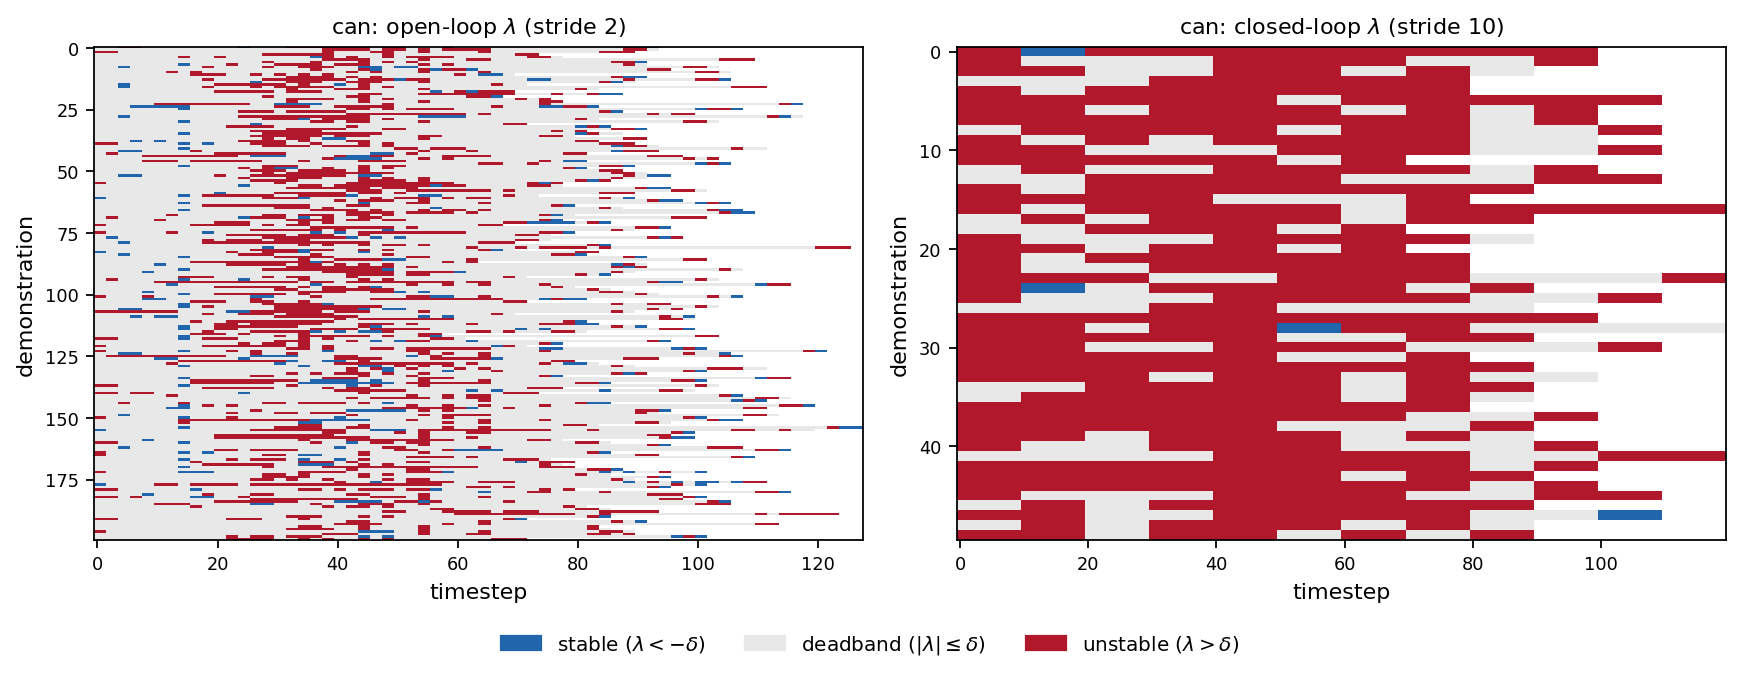
\includegraphics[width=0.98\linewidth]{figs/timeline_can.png}\\[2pt]
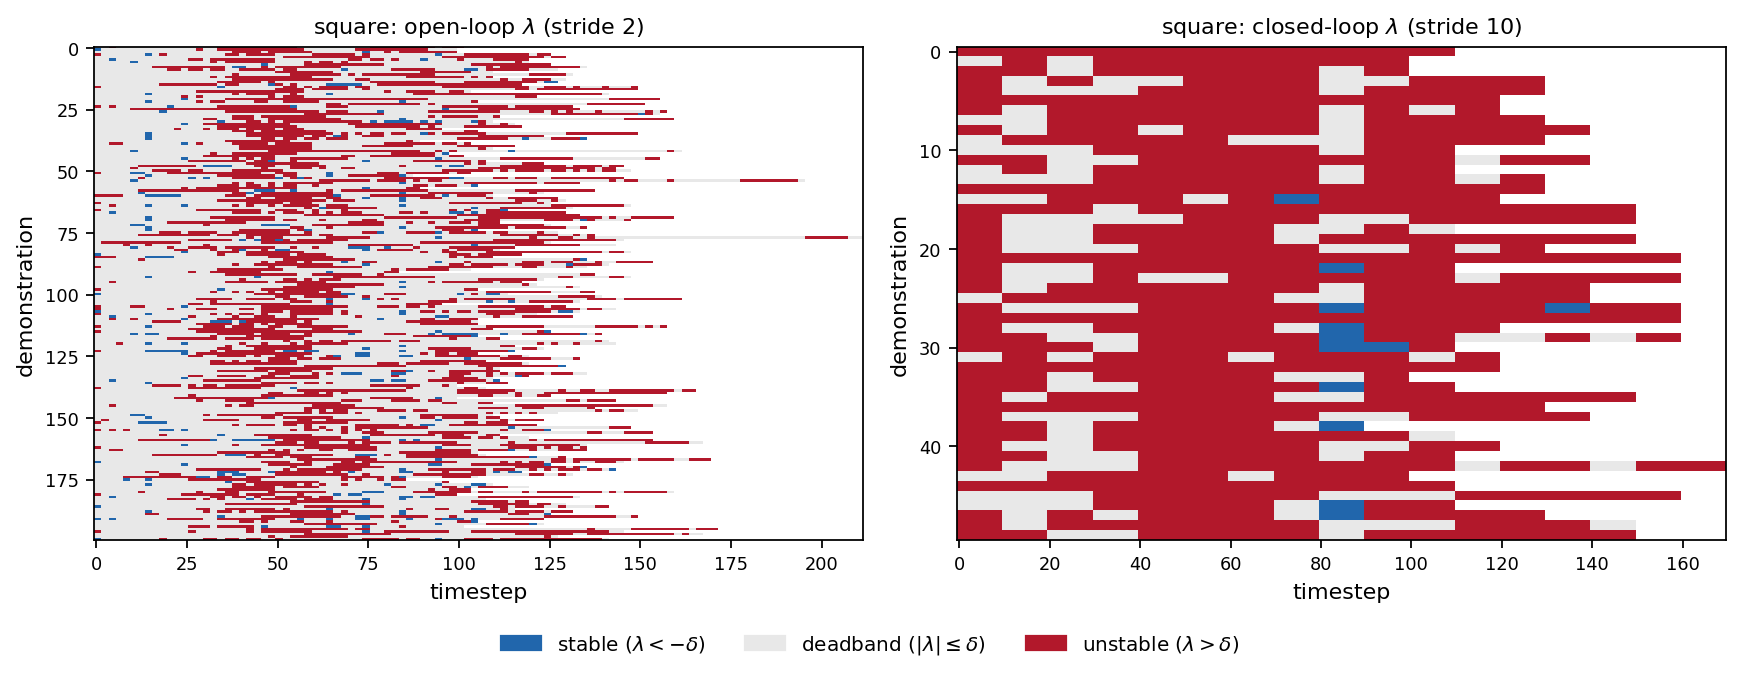
\includegraphics[width=0.98\linewidth]{figs/timeline_square.png}\\[2pt]
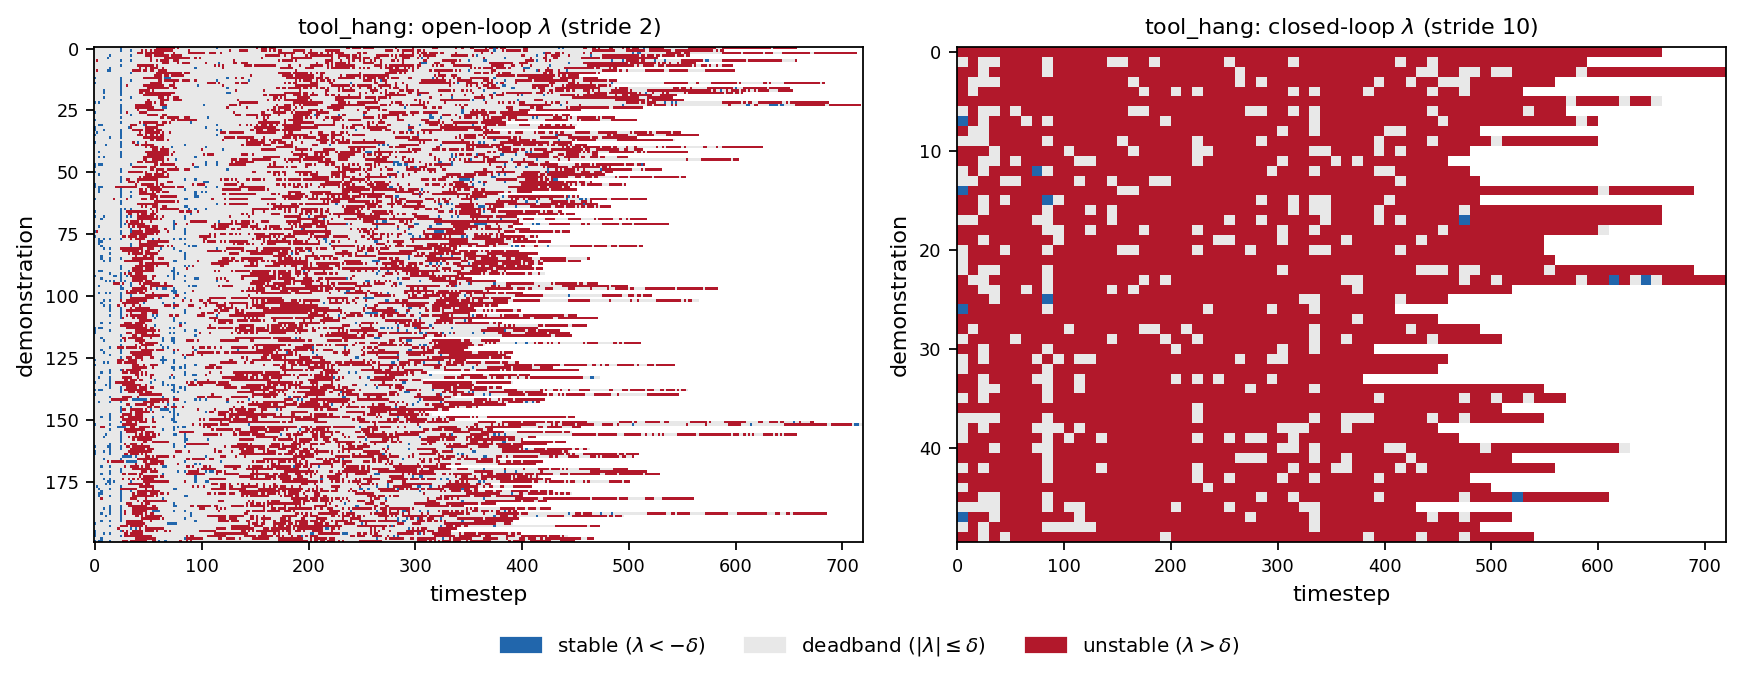
\includegraphics[width=0.98\linewidth]{figs/timeline_tool_hang.png}
\end{center}

Contiguity, quantified (a run is a maximal stretch of consecutive same-class
stamps within one demonstration; lengths are converted to environment steps):

\begin{center}
\footnotesize
\begin{tabular}{@{}llccccc@{}}
\toprule
Task & Ch. & occupancy s/d/u & mean run & median run &
trans./demo & mass in runs $\geq$3 \\
\midrule
lift       & OL & .00/.75/.25 & 11 & 8  & 1.2  & 0.94 \\
can        & OL & .04/.75/.20 & 9  & 4  & 9.8  & 0.82 \\
square     & OL & .03/.63/.34 & 10 & 4  & 11.9 & 0.86 \\
tool\_hang & OL & .02/.58/.40 & 9  & 4  & 52.0 & 0.83 \\
\addlinespace
lift       & CL & .00/.14/.86 & 22 & 20 & 0.4  & 0.64 \\
can        & CL & .01/.30/.69 & 23 & 20 & 3.2  & 0.60 \\
square     & CL & .02/.23/.75 & 27 & 20 & 3.8  & 0.69 \\
tool\_hang & CL & .00/.14/.86 & 43 & 20 & 11.6 & 0.82 \\
\bottomrule
\end{tabular}
\end{center}

What the timelines show, honestly stated:

\begin{enumerate}[leftmargin=2em]
  \item \textbf{The labels have real long-horizon structure at the phase
        level.} Every task shows the same macro-pattern, aligned across
        demonstrations: an early deadband band during the approach (clearly
        visible as the gray column on square before step 30 and on tool\_hang
        before step 100), then unstable segments through the
        contact-rich manipulation phases. This is task structure, not noise,
        and it is what a switch needs to exist.
  \item \textbf{They are not salt and pepper, but boundaries flicker.} 82 to
        94 percent of open-loop stamp mass sits in runs of three or more
        stamps (six or more steps). The median open-loop run is still short
        (4 steps on can, square, and tool\_hang), and tool\_hang averages 52
        class transitions per demonstration, so within the contact phase the
        signal alternates at the few-stamp scale. This is exactly the
        behavior the deadband, the median filter, and the rollout-time
        hysteresis were designed to absorb, and it is why raw stamps should
        never be consumed without one of those mechanisms.
  \item \textbf{True stable stamps are rare; the practical contrast is
        deadband versus unstable.} Only 0 to 4 percent of open-loop stamps
        fall below $-\delta$. The switch's ``stable'' regime in practice is
        the deadband, which is consistent with how the threshold was chosen
        ($\delta$ at the 95th percentile of the below-median magnitudes).
  \item \textbf{The closed-loop channel is near-uniformly expansive, in
        blocks.} The CL panels are mostly red with isolated deadband stamps,
        matching the 90 to 99 percent positive rates reported above; with
        only about 54 stamps per demonstration at stride 10, its timelines
        carry coarser information than the open-loop ones.
\end{enumerate}

One connection to the rollout experiments is worth recording here. The
timelines bound how much an oracle or predictor switch can matter: on
tool\_hang the oracle-switched rollout cells spent only about 16 percent of
their steps in the stable mode (44 percent on square, derived from the
recorded mean executed $k$), yet every single rollout episode mixed both
modes. The switching signal fires; what limits its value on these tasks is the
lopsided occupancy, not a failure to switch.

%=====================================================================
\section{Sanity-check assets: what exists and how to read it}

All artifacts live under \texttt{results/label\_videos/} in the project root
(\texttt{long-horizon/}), one folder per dataset.

\subsection{Annotated demo videos}

Files: \texttt{results/label\_videos/<dataset>/demo\_<i>.mp4}, five demos per
dataset, for: lift, can, square, tool\_hang, mg\_stack\_d0, mg\_square\_d0, and each
finished LIBERO file (prefix \texttt{libero10\_}). Each video replays the
demonstration in the simulator with a colored border per frame:

\begin{itemize}[leftmargin=2em]
  \item \textbf{Red}: the active label at that frame is unstable
        ($\lambda > +\delta$).
  \item \textbf{Green}: stable ($\lambda < -\delta$).
  \item \textbf{Gray}: deadband (unproven; resolved later by neighbor inheritance).
\end{itemize}

Figure~\ref{fig:frames} shows red and gray example frames from four datasets.

The top bar prints the current $\lambda$, the verdict, and the window contact flags
\texttt{c[g t f]} (gripper / table / fixture). Labels are forward-looking: the color
at frame $t$ describes the window $[t, t{+}24)$. What to check when watching: the
border should turn red at grasps, insertions, and placements, and stay gray during
transport. A \texttt{README.json} in each folder repeats the legend.

\subsection{Divergence-curve graphs}

Files, three most-contractive and three most-expansive stamps per dataset, selected
from distinct demos:\\
\texttt{results/label\_videos/<dataset>/divergence\_curves/}\\
\texttt{\{stable,unstable\}\_<rank>\_demo<id>\_t<t0>.png}\\
A \texttt{selection.json} beside them lists each stamp with its label and recomputed
$\lambda$. Each graph shows the probe at one stamp:

\begin{itemize}[leftmargin=2em]
  \item Thin gray lines: $\lVert x^{pert}(\tau) - x^{nom}(\tau) \rVert$ for each of
        the 8 perturbed branches, on a log scale, over the 24-step window.
  \item Bold blue line: the branch mean. Dashed orange line: the fitted exponential
        whose slope is $\lambda$. Dotted horizontal line: the injected size
        $\sigma_u$.
\end{itemize}

Reading: in an expansive stamp the fan of gray lines climbs (the error funnels out);
in a contractive stamp it falls back toward zero (the error funnels in); in a
neutral stamp it stays flat near the $\sigma_u$ line. These graphs are the direct
visual form of the quantity the label thresholds. Figure~\ref{fig:curves} shows four
representative examples.

\begin{figure}[p]
\centering
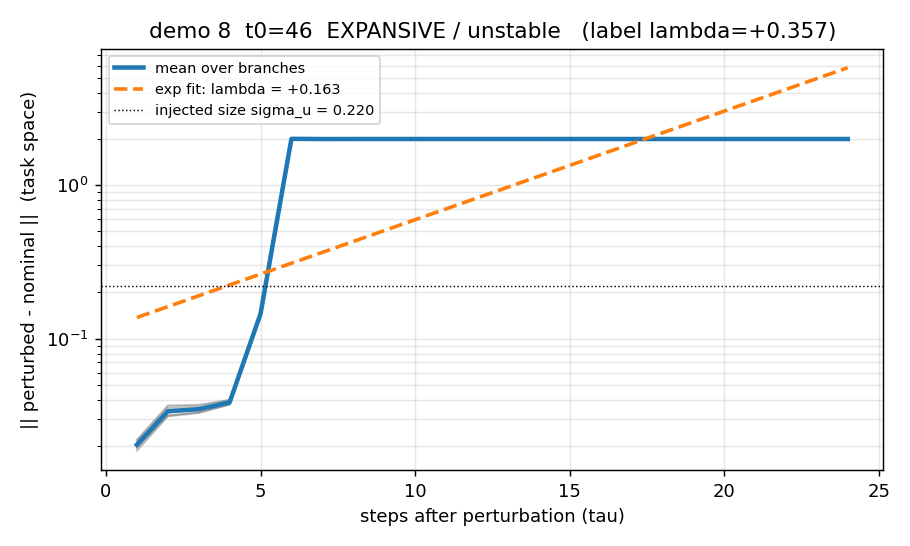
\includegraphics[width=0.49\linewidth]{figs/curve_square_unstable_0.png}
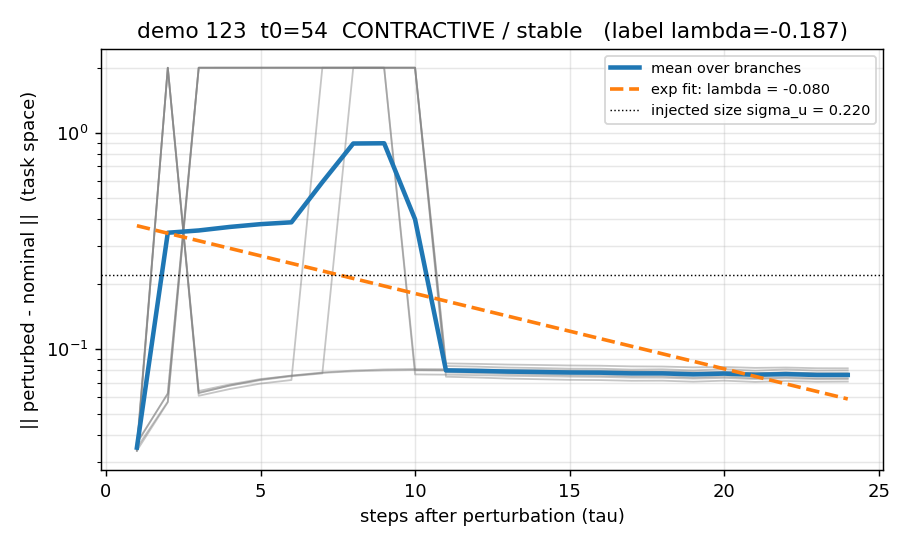
\includegraphics[width=0.49\linewidth]{figs/curve_square_stable_0.png}\\[2pt]
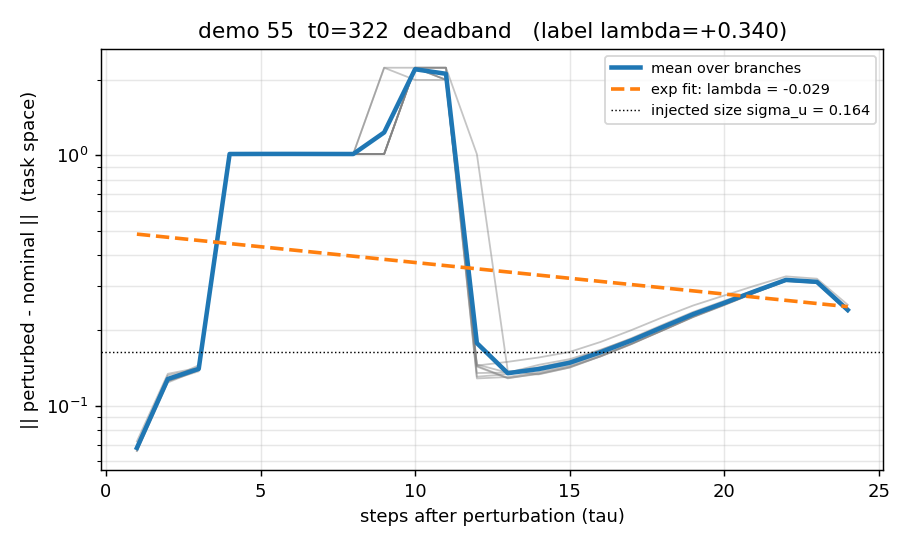
\includegraphics[width=0.49\linewidth]{figs/curve_tool_hang_unstable_0.png}
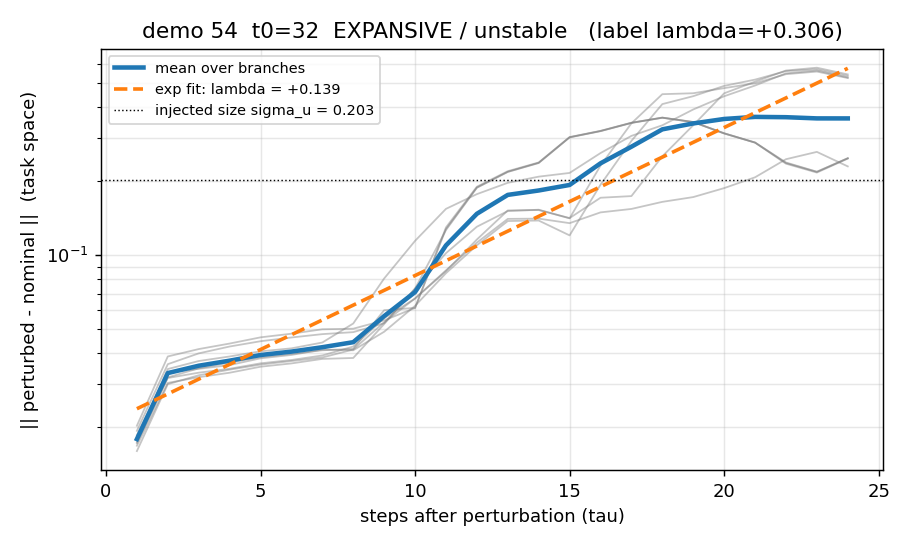
\includegraphics[width=0.49\linewidth]{figs/curve_mg_stack_d0_unstable_0.png}
\caption{Divergence curves at four labeled stamps: perturbed-versus-nominal error
over the 24-step window, log scale. Thin gray lines are the 8 individual perturbed
branches, blue is their mean, dashed orange is the fitted exponential whose slope is
$\lambda$, and the dotted horizontal line marks the injected size $\sigma_u$.
Top left: square at its most expansive stamp; the error fans out by more than an
order of magnitude, the funnel opens. Top right: square at its most contractive
stamp; the branches fall back toward the nominal trajectory, the funnel closes.
Bottom left: tool\_hang at an expansive contact stamp. Bottom right: MimicGen
stack\_d0 at its most expansive stamp (cube placement); generated demos produce the
same signature as human ones.}
\label{fig:curves}
\end{figure}

\begin{figure}[p]
\centering
\begin{tabular}{@{}cc@{}}

\includegraphics[width=0.42\linewidth]{figs/frame_square_red.png} &
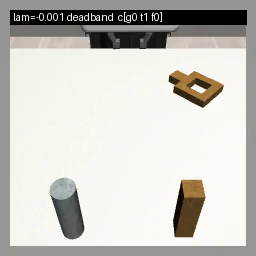
\includegraphics[width=0.42\linewidth]{figs/frame_square_gray.png} \\
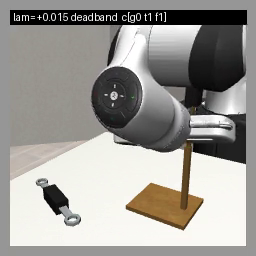
\includegraphics[width=0.42\linewidth]{figs/frame_tool_hang_red.png} &
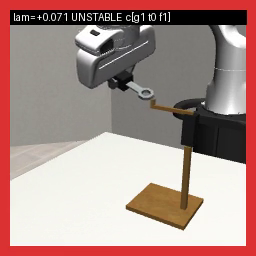
\includegraphics[width=0.42\linewidth]{figs/frame_tool_hang_gray.png} \\
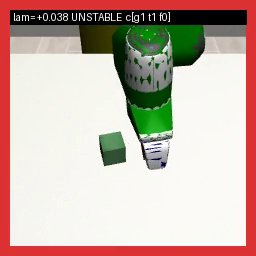
\includegraphics[width=0.42\linewidth]{figs/frame_mg_stack_d0_red.png} &
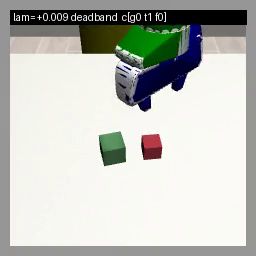
\includegraphics[width=0.42\linewidth]{figs/frame_mg_stack_d0_gray.png} \\
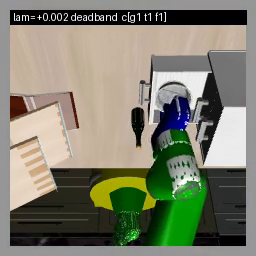
\includegraphics[width=0.42\linewidth]{figs/frame_libero10_KITCHEN_SCENE4_put_the_black_bowl_in_the_red.png} &
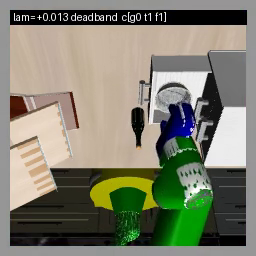
\includegraphics[width=0.42\linewidth]{figs/frame_libero10_KITCHEN_SCENE4_put_the_black_bowl_in_the_gray.png}
\end{tabular}
\caption{Frames from the annotated sanity videos. Left column: the most expansive
labeled stamp of the first rendered demo (red border, label unstable). Right column:
the most neutral stamp of the same demo (gray border, deadband). Rows: square,
tool\_hang, MimicGen stack\_d0, LIBERO bowl-in-cabinet. The top bar of each frame
prints the current $\lambda$, the verdict, and the window contact flags. Note the
red frames are grasp, insertion, or placement moments and the gray frames are
transport or pre-contact moments, which is the qualitative alignment the AUROC
numbers quantify.}
\label{fig:frames}
\end{figure}

%=====================================================================
\section{Caveats and open items}
\label{sec:caveats}

\begin{enumerate}[leftmargin=2em]
  \item \textbf{LIBERO labels are provisional.} Interim $\sigma_u$ (borrowed
        robomimic mean) and generic contact patterns; contact-alignment AUROC 0.42
        to 0.63 where computable, and not computable at all in the six scenes where
        the generic patterns register contact in every window (those scenes also
        use the suite-fallback $\delta = 0.019$). Fix: per-scene task-object
        patterns for the sanity channel, and a measured $\sigma_u$ once a LIBERO
        policy is trained. All ten files are labeled.
  \item \textbf{MimicGen $\sigma_u$ is borrowed} (square-ph value and robomimic
        mean). Defensible for same-embodiment same-controller data, but should be
        re-measured when policies are trained on MimicGen tasks.
  \item \textbf{Closed-loop coverage stops at the four robomimic tasks.} All
        four sets are done (tool\_hang took 53.6 hours of wall-clock). MimicGen
        and LIBERO have no closed-loop channel yet; adding one costs about a
        policy-inference-day per task and is not currently scheduled.
  \item \textbf{can has no free-space stamps} by construction, so its AUROC is
        undefined and its $\delta$ is a fallback. Optional refinement: count
        object-resting-with-gripper-far as quasi-free for the noise floor.
  \item \textbf{Contact flags are sanity only.} They never enter the labels. All
        alignment numbers here are checks of plausibility, not training targets.
  \item \textbf{FurnitureSim is blocked} on a manual Isaac Gym download.
  \item \textbf{Deadband dominates} (61--86\%). This is expected physics (see
        Pattern 2) and is handled by neighbor inheritance, but it means the
        predictor's decision boundary rests on roughly a quarter to a third of
        stamps being confidently labeled. Class weighting in the BCE loss is
        already planned for this.
\end{enumerate}

%=====================================================================
\section{Summary}

Sixteen datasets and about 155{,}000 open-loop stamps are labeled with a
verified-deterministic perturb-and-replay FTLE probe, using measured policy error
sizes wherever a trained policy exists, plus three finished closed-loop sets. The
labels behave the way the hypothesis needs them to: contact-heavy moments are
systematically the most expansive, the mostly-stable control task is measurably the
most benign, generated demos mirror human demos, and the closed-loop channel shows
policy feedback amplifying error exactly where the plant alone would not, now on
three tasks (99.3\%, 90.4\%, and 93.0\% of stamps positive on lift, can, and
square). The visual sanity layer (annotated videos and divergence graphs) exists
for every finished dataset, including all ten LIBERO files. The open-loop labels
have since fed the first predictor trainings and the Stage 1a evaluation, which are
documented separately.

\end{document}
